% !TeX spellcheck = es_ES
\documentclass[12pt]{article}
\usepackage[utf8]{inputenc}
\usepackage[spanish]{babel}
\usepackage{graphicx}
\usepackage[margin=2.5cm]{geometry}
\usepackage{float}
\usepackage{amsmath}
\usepackage{amsfonts}
\usepackage{booktabs}
\usepackage{hyperref}

\hypersetup{
	colorlinks=true,
	linkcolor=black,
	urlcolor=blue,
	citecolor=blue
}

\newcommand{\hrules}{\rule{\linewidth}{0.5mm}}

\begin{document}
	
	\begin{titlepage}
		\centering
		
		\begin{minipage}{0.2\textwidth}
			\begin{flushleft}
				
\includegraphics[width=\textwidth]{logo_ipn.png}
			\end{flushleft}
		\end{minipage}
		\hfill
		\begin{minipage}{0.5\textwidth}
			\centering
			{\scshape\Large Instituto Politécnico Nacional} \\[0.3cm]
			{\scshape\large Escuela Superior de Cómputo}
		\end{minipage}
		\hfill
		\begin{minipage}{0.2\textwidth}
			\begin{flushright}
				
\includegraphics[width=\textwidth]{logo_escom.png}
			\end{flushright}
		\end{minipage}
		
		\vspace{1.5cm}
		
		{\large\textbf{Ingeniería en Inteligencia Artificial}} \\[1.5cm]
		
		{\Large\textbf{Redes Neuronales y Aprendizaje Profundo}} \\[2cm]
		
		\hrules
		\vspace{0.4cm}
		{\huge\bfseries 
			Práctica 2: Perceptrón Multicapa 
		} \\[0.4cm]
		\hrules
		\vspace{2.5cm}
		
		% --- INFORMACIÓN PERSONAL ---
		\begin{minipage}{0.8\textwidth}
			\begin{flushleft} \large
				\textbf{Profesor:} \\
				Saúl de la O Torres 
				\\[1cm]
				
				\textbf{Alumno:} \\
				Velázquez Arrieta Eduardo Uriel
			\end{flushleft}
		\end{minipage}
		
		\vfill
	\end{titlepage}
	
	\newpage
	\tableofcontents % Índice de contenido
	\vspace{1cm}
	\listoffigures    % Índice de imágenes
	\newpage
	
	\section{Introducción}
	El Perceptrón Simple propuesto por Frank Rosenblatt sentó las bases del aprendizaje supervisado conexionista; sin embargo, presentó una limitación teórica trascendental demostrada por Minsky y Papert en 1969: la incapacidad de resolver problemas no linealmente separables, como la función lógica XOR. La superación de este cuello de botella derivó en la arquitectura del Perceptrón Multicapa (\textit{Multilayer Perceptron}, MLP), el cual incorpora una o más capas ocultas dotadas de funciones de activación no lineales (como ReLU y Sigmoide) y algoritmos de optimización basados en el descenso de gradiente mediante retropropagación (\textit{backpropagation}).
	
	El objetivo primordial de esta práctica es analizar, implementar y optimizar redes neuronales densamente conectadas bajo un enfoque modular y orientado a objetos en Python utilizando TensorFlow/Keras. Para ello se cubren los siguientes objetivos específicos:
	\begin{enumerate}
		\item \textbf{Modelado Modular}: Diseñar clases que encapsulen la instanciación de capas, optimizadores, rutinas de entrenamiento y mecanismos de evaluación.
		\item \textbf{Separabilidad Lógica}: Demostrar la convergencia del MLP en compuertas linealmente separables (AND, OR) y no linealmente separables (XOR).
		\item \textbf{Investigación de Conjuntos de Datos}: Analizar datasets de referencia como Fashion-MNIST y CIFAR-10, evaluando la dimensionalidad de las muestras y la complejidad de clasificación asociada a imágenes a escala de grises y a color RGB.
		\item \textbf{Sensibilidad de Hiperparámetros}: Modificar topologías (profundidad, número de unidades ocultas, tasas de aprendizaje y capas de regularización) para identificar fenómenos de subajuste (\textit{underfitting}) y sobreajuste (\textit{overfitting}).
		\item \textbf{Optimización y Desempeño}: Desarrollar una arquitectura capaz de superar el umbral basal del 47\% de precisión en la clasificación multiclase sobre el conjunto CIFAR-10.
	\end{enumerate}
	
	\subsection{Descripción de los Conjuntos de Datos}
	\begin{itemize}
		\item \textbf{Fashion-MNIST}: Introducido por Zalando Research como un reemplazo directo y más desafiante que el clásico MNIST. Consta de 70,000 imágenes en escala de grises de $28 \times 28$ píxeles distribuidas equitativamente en 10 categorías de prendas y calzado (60,000 de entrenamiento y 10,000 de prueba).
		\item \textbf{CIFAR-10}: Recopilado por Alex Krizhevsky, Vinod Nair y Geoffrey Hinton, este dataset comprende 60,000 imágenes a color de $32 \times 32$ píxeles con 3 canales (RGB), divididas en 10 clases mutuamente excluyentes (avión, automóvil, pájaro, gato, venado, perro, rana, caballo, barco y camión). Representa un reto substancial para un MLP debido a la dimensionalidad plana de entrada ($32 \times 32 \times 3 = 3072$ características) y la ausencia de invariancia traslacional intrínseca a capas totalmente conectadas.
	\end{itemize}
	
	\section{Desarrollo}
	La implementación se estructuró en tres módulos principales dentro de Jupyter Notebook - Google Colab:
	
	\subsection{Adaptación del código a clases}
	Para probar y variar los parámetros de la red neuronal se crearon clases para cada uno de los códigos; esto con el objetivo de reutilizar el mismo código y solo cambiar los parámetros de entrada.
	
	\subsubsection{Perceptrón multicapa para varias compuertas}
	Como se logra observar en la Figura 1, el código uno no es con base en objetos y solo clasifica con la compuerta \textbf{XOR}, algo que es posible gracias a que ya contamos con varios perceptrones.
	
	\begin{figure}[H]
		\centering
		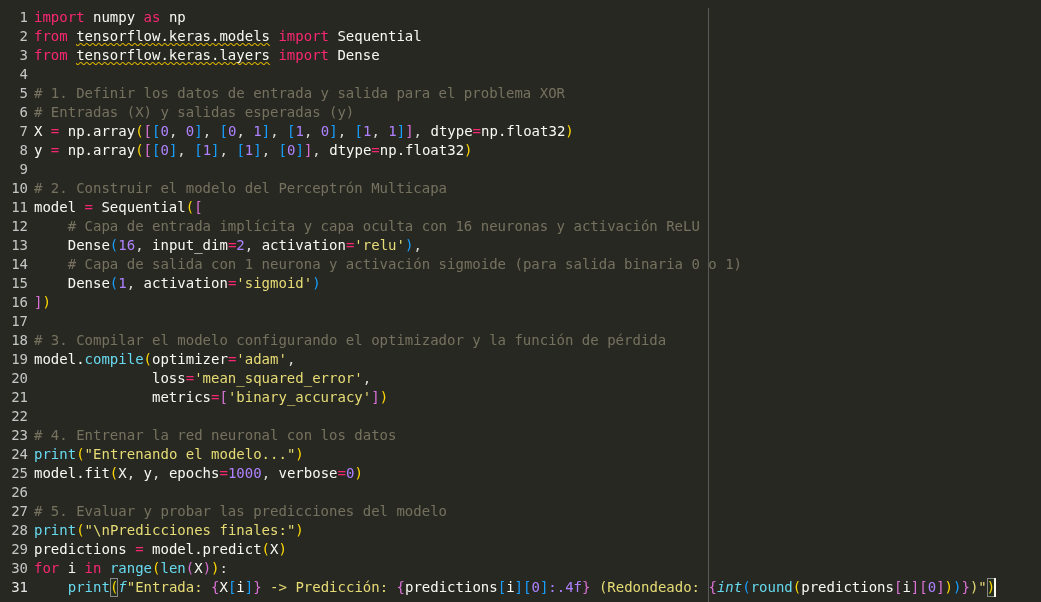
\includegraphics[width=0.7\textwidth]{img1.png} 
		\caption{Código 1 original.}
		\label{fig:esquema_2}
	\end{figure}
	
	
	Como se aprecia en la Figura 2, ahora el código si es con base en objetos y además ya puede clasificar las tres compuertas \textbf{XOR}, \textbf{AND} y 
	\textbf{OR}. \\ 
	Una de las principales diferencias que podemos observar es que ya contamos con métodos para poder crear varias instancias de la misma clase; además de que podemos escoger con que compuerta queremos trabajar.
	
	
		\begin{figure}[H]
		\centering
		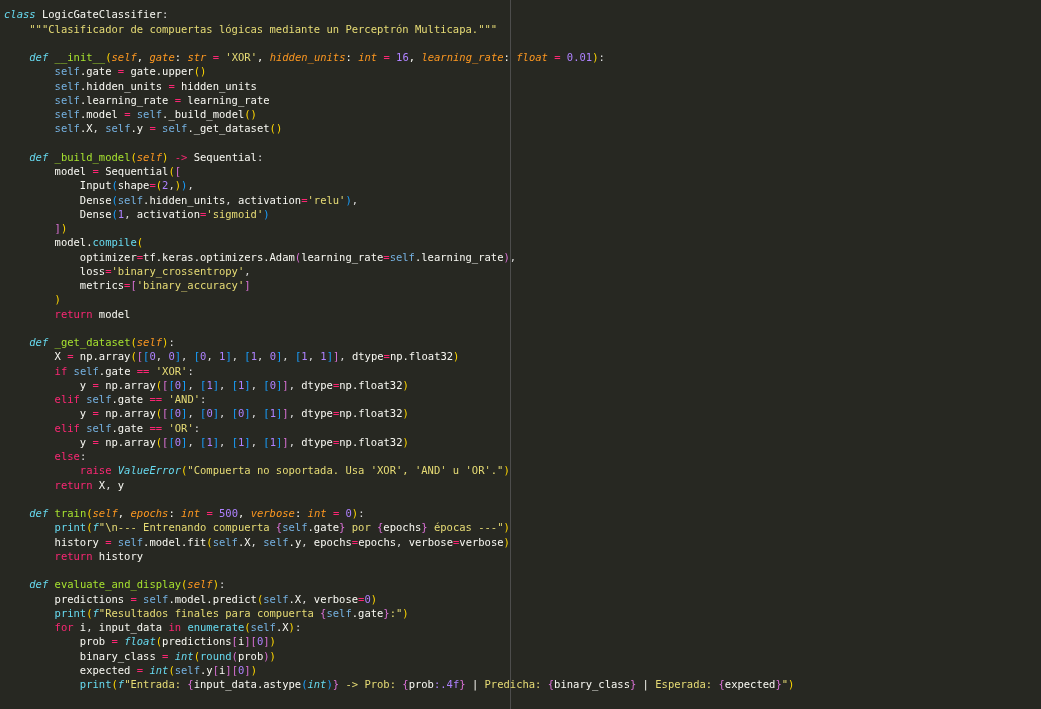
\includegraphics[width=0.7\textwidth]{img2.png} 
		\caption{Código 2 (modificado y con base en objetos).}
		\label{fig:esquema_3}
	\end{figure}	
	
	
	
	\subsubsection{Perceptrón multicapa para clasificación de imágenes en escala de grises}
	Como se observa en la Figura 3, solo podemos entrenar la red para clasificar las imágenes con ciertos parámetros en especifico, lo que vuelve el código difícil de usar y poco práctico.
	
	\begin{figure}[H]
		\centering
		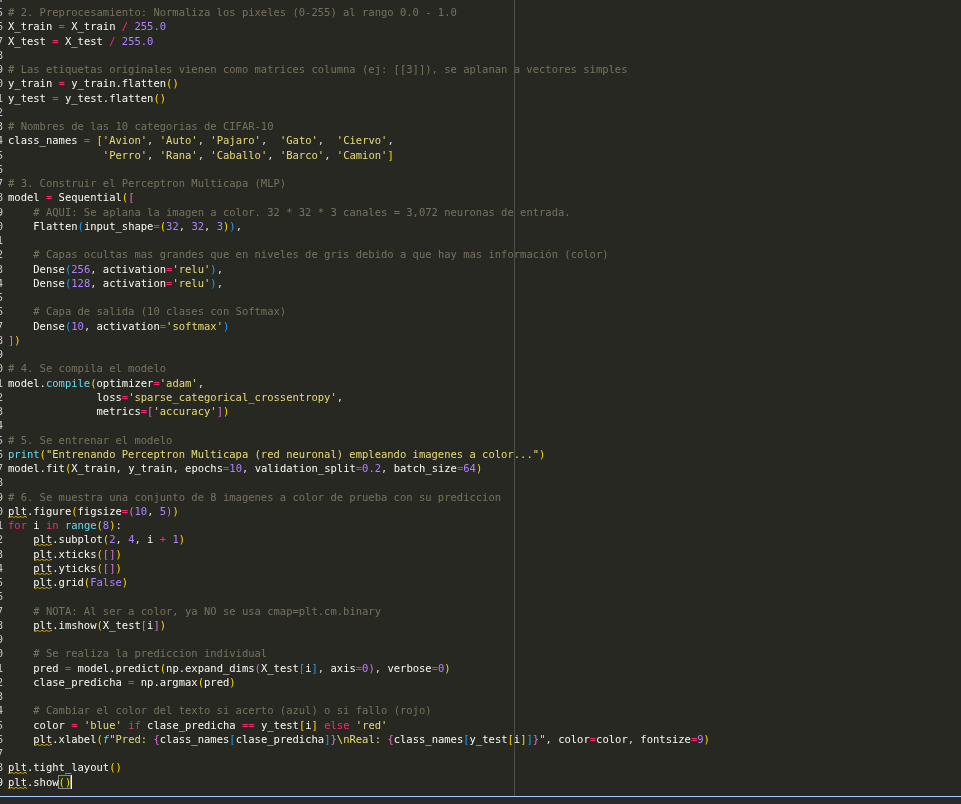
\includegraphics[width=0.7\textwidth]{img3.png} 
		\caption{Código 2 original.}
		\label{fig:esquema4}
	\end{figure}	
	
	
	En la Figura 4 notamos que tiene mucho más sentido usar \textbf{POO} para poder entrenar variando los parámetros, algo fundamental en el mundo del \textbf{Deep Learning}, ya que puede existir la posibilidad de que si no usamos las épocas o capas suficientes el modelo tenga \textbf{Underfitting} o en caso contrario si tenemos muchas épocas y capas podemos obtener \textbf{Overfitting} y un gasto completamente innecesario de recursos.
	
	
	\begin{figure}[H]
		\centering
		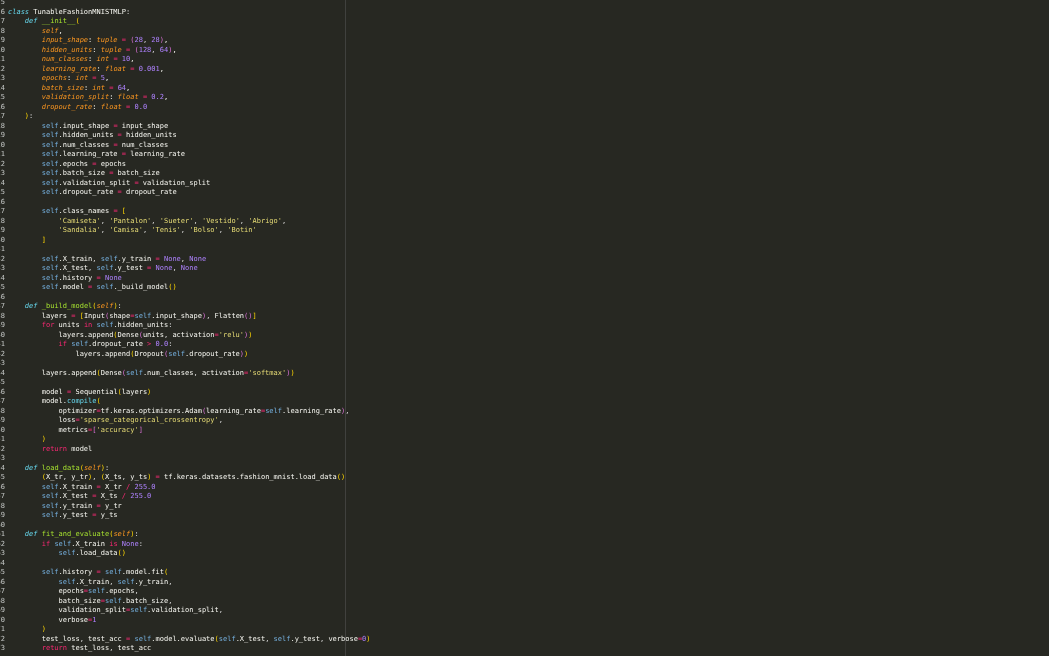
\includegraphics[width=0.7\textwidth]{img4.png} 
		\caption{Código 2 (Modificado y orientado a objetos).}
		\label{fig:esquema5}
	\end{figure}	
		
	También tenemos las pruebas; este fragmento de código nos sirve para entrenar el modelo con varios parámetros y obtener la mejor combinación de parámetros posible.
	
	
	\begin{figure}[H]
		\centering
		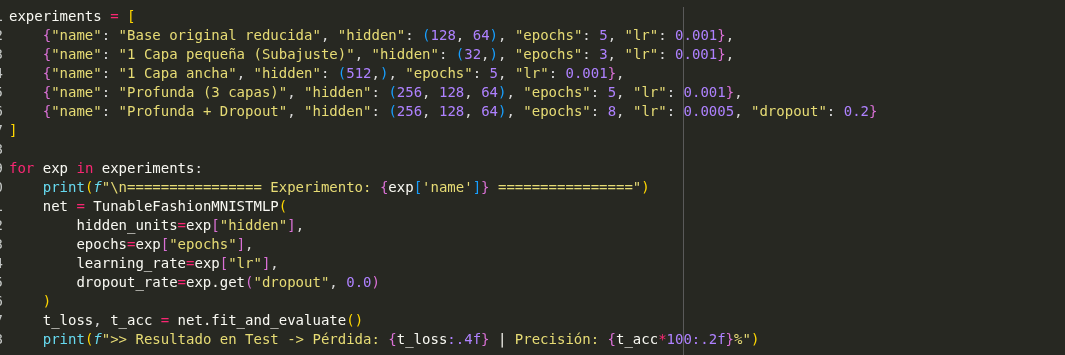
\includegraphics[width=0.7\textwidth]{img5.png} 
		\caption{Código 3 Validación de parámetros.}
		\label{fig:esquema6}
	\end{figure}	
	

	\subsubsection{Perceptrón multicapa para clasificación de imágenes a color}
	
	Para la clasificación con imágenes a color tenemos básicamente el mismo problema que con las que son a blanco y negro, no podemos evaluar con varios parámetros lo que vuelve el código difícil y poco práctico de usar.
	
	
	
	\begin{figure}[H]
		\centering
		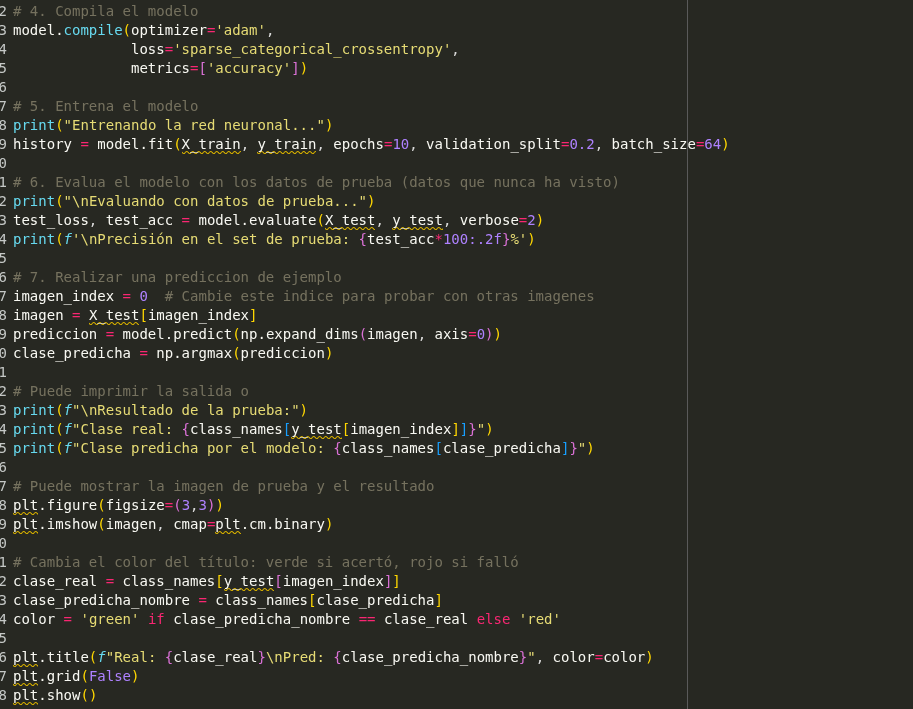
\includegraphics[width=0.7\textwidth]{img6.png} 
		\caption{Código 4 original.}
		\label{fig:esquema7}
	\end{figure}	
	
	Ahora con el paradigma orientado a objetos podemos generar varios objetos para obtener diferentes resultados y tratar de mejorar el accuracy de \textbf{\%49}.
	
	
	\begin{figure}[H]
		\centering
		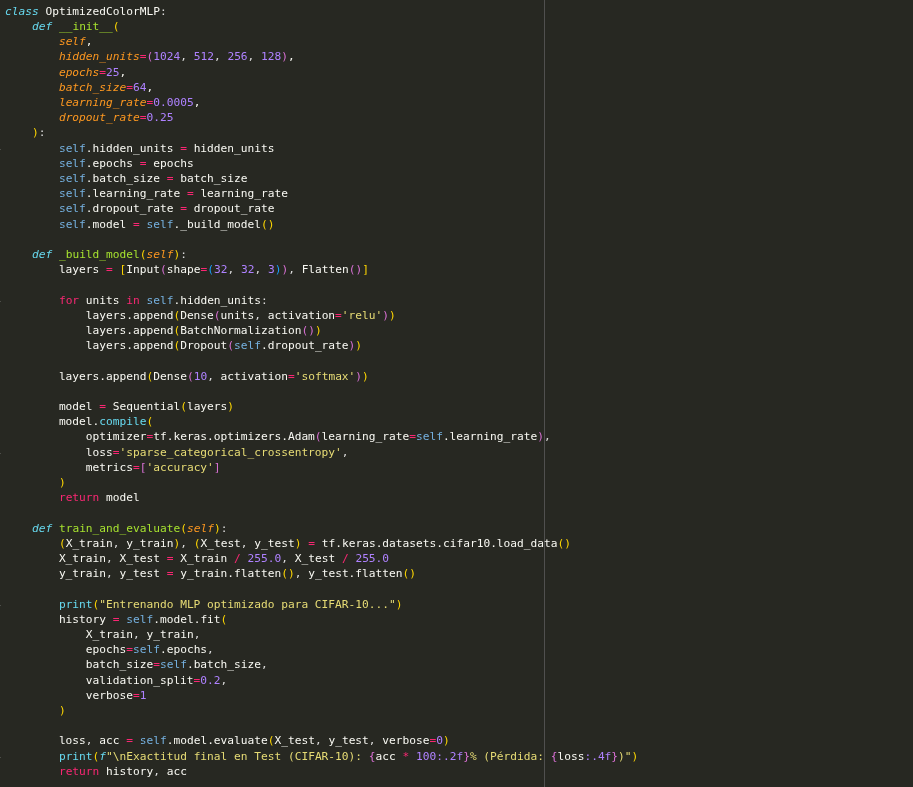
\includegraphics[width=0.7\textwidth]{img7.png} 
		\caption{Código 4 (Modificado y orientado a objetos).}
		\label{fig:esquema8}
	\end{figure}	
	
	
	
	
	\subsection{Módulo 1: Clasificador de Compuertas Lógicas (\texttt{LogicGateClassifier})}
	Se implementó una clase modular para mapear las relaciones booleanas de dos entradas $X \in \{0, 1\}^2$ a una salida $y \in \{0, 1\}$.
	\begin{itemize}
		\item \textbf{Arquitectura}: Capa de entrada de dimensionalidad 2, capa oculta con $8$ a $16$ unidades y función de activación ReLU, seguida de una neurona de salida con activación sigmoide:
		\begin{equation}
			\sigma(z) = \frac{1}{1 + e^{-z}}
		\end{equation}
		\item \textbf{Función de Pérdida}: Entropía cruzada binaria (\textit{Binary Cross-Entropy}):
		\begin{equation}
			\mathcal{L} = -\frac{1}{N}\sum_{i=1}^{N} \left[ y_i \log(\hat{y}_i) + (1 - y_i)\log(1 - \hat{y}_i) \right]
		\end{equation}
		\item \textbf{Optimizador}: Adam con tasa de aprendizaje $\eta = 0.05$ por 300 épocas.
	\end{itemize}
	
	\subsection{Módulo 2: Clasificación en Escala de Grises (\texttt{TunableFashionMNISTMLP})}
	Se diseñó una arquitectura flexible para clasificar prendas a partir de tensores bidimensionales ($28 \times 28$):
	\begin{itemize}
		\item \textbf{Preprocesamiento}: Normalización Min-Max de las intensidades de los píxeles a un rango continuo en $[0, 1]$ dividiendo por $255.0$.
		\item \textbf{Vectorización}: Capa \texttt{Flatten} para convertir matrices $28 \times 28$ a vectores de 784 componentes.
		\item \textbf{Capas Densas y Regularización}: Posibilidad de definir capas intermedias arbitrarias, regularización por descarte (\texttt{Dropout}) y capa de salida de 10 unidades con función de activación \textit{Softmax}:
		\begin{equation}
			\text{Softmax}(z_j) = \frac{e^{z_j}}{\sum_{k=1}^{10} e^{z_k}}
		\end{equation}
		\item \textbf{Experimentación Sistemática}: Se evaluaron cinco configuraciones:
		\begin{enumerate}
			\item \textit{Base original reducida}: $(128, 64)$ unidades, 5 épocas, $\eta = 0.001$.
			\item \textit{1 Capa pequeña (Subajuste)}: $(32)$ unidades, 3 épocas, $\eta = 0.001$.
			\item \textit{1 Capa ancha}: $(512)$ unidades, 5 épocas, $\eta = 0.001$.
			\item \textit{Profunda (3 capas)}: $(256, 128, 64)$ unidades, 5 épocas, $\eta = 0.001$.
			\item \textit{Profunda + Dropout}: $(256, 128, 64)$ unidades, \textit{Dropout} de $0.2$, 8 épocas, $\eta = 0.0005$.
		\end{enumerate}
	\end{itemize}
	
	\subsection{Módulo 3: Optimización para Imágenes a Color (\texttt{OptimizedColorMLP})}
	Para abordar CIFAR-10 y superar la barrera del 47\% de exactitud con un perceptrón multicapa, se elaboró una topología profunda y regularizada:
	\begin{itemize}
		\item \textbf{Vectorización}: Entrada de $32 \times 32 \times 3$, aplanada a 3072 entradas continuas.
		\item \textbf{Topología}: Secuencia de 4 bloques densos decrecientes: $1024 \to 512 \to 256 \to 128$ unidades ReLU.
		\item \textbf{Normalización por Lotes y Regularización}: Tras cada capa lineal se integró \texttt{BatchNormalization} para estabilizar la distribución de las activaciones intermedias y contrarrestar el cambio de covariable interno, junto a un \texttt{Dropout} de $0.25$ para mitigar la coadaptación de neuronas.
		\item \textbf{Entrenamiento}: Optimizador Adam con $\eta = 0.0003$, batch size de 64, split de validación del 20\% y 20 épocas de entrenamiento.
	\end{itemize}
	
	\section{Resultados Obtenidos}
	
	\subsection{Compuertas Lógicas}
	Los resultados de salida para cada compuerta lógica tras 300 épocas se detallan a continuación:
	
	\begin{table}[H]
		\centering
		\caption{Resultados obtenidos por el MLP en compuertas lógicas.}
		\begin{tabular}{ccccc}
			\toprule
			\textbf{Compuerta} & \textbf{Entrada} & \textbf{Probabilidad Obtenida} & \textbf{Predicción} & \textbf{Esperado} \\
			\midrule
			AND & $[0, 0]$ & 0.0000 & 0 & 0 \\
			AND & $[0, 1]$ & 0.0143 & 0 & 0 \\
			AND & $[1, 0]$ & 0.0003 & 0 & 0 \\
			AND & $[1, 1]$ & 0.9990 & 1 & 1 \\
			\midrule
			OR  & $[0, 0]$ & 0.0189 & 0 & 0 \\
			OR  & $[0, 1]$ & 0.9998 & 1 & 1 \\
			OR  & $[1, 0]$ & 0.9997 & 1 & 1 \\
			OR  & $[1, 1]$ & 1.0000 & 1 & 1 \\
			\midrule
			XOR & $[0, 0]$ & 0.0052 & 0 & 0 \\
			XOR & $[0, 1]$ & 0.9994 & 1 & 1 \\
			XOR & $[1, 0]$ & 0.9993 & 1 & 1 \\
			XOR & $[1, 1]$ & 0.0052 & 0 & 0 \\
			\bottomrule
		\end{tabular}
	\end{table}
	
	\subsection{Comparativa en Fashion-MNIST}
	La exploración de hiperparámetros en Fashion-MNIST produjo las siguientes métricas sobre el conjunto de prueba independiente (10,000 imágenes):
	
	\begin{table}[H]
		\centering
		\caption{Comparativa experimental de arquitecturas MLP en Fashion-MNIST.}
		\begin{tabular}{lcccc}
			\toprule
			\textbf{Configuración} & \textbf{Capas Ocultas} & \textbf{Épocas} & \textbf{Pérdida (Test)} & \textbf{Precisión (\%)} \\
			\midrule
			1. Subajuste            & $(32)$               & 3 & 0.4197 & 85.57\% \\
			2. 1 Capa Ancha         & $(512)$              & 5 & 0.3816 & 86.18\% \\
			3. Profunda (3 capas)   & $(256, 128, 64)$     & 5 & 0.3636 & 86.67\% \\
			4. Base reducida        & $(128, 64)$          & 5 & 0.3647 & 87.30\% \\
			5. Profunda + Dropout   & $(256, 128, 64)$     & 8 & \textbf{0.3492} & \textbf{87.44\%} \\
			\bottomrule
		\end{tabular}
	\end{table}
	
	\subsection{Optimización en CIFAR-10}
	El modelo \texttt{OptimizedColorMLP} logró romper el límite base del 47\%, manteniendo un aprendizaje constante a lo largo de las 20 épocas de cómputo. En la última época se registraron las siguientes métricas de entrenamiento:
	\begin{itemize}
		\item \textbf{Entrenamiento (Época 20)}: Pérdida: $1.4129$, Exactitud: $49.60\%$.
		\item \textbf{Validación (Época 20)}: Pérdida: $1.4440$, Exactitud: $49.03\%$.
		\item \textbf{Conjunto de Prueba Final}: Pérdida: \textbf{1.4289}, Exactitud: \textbf{49.65\%}.
	\end{itemize}
	
	El estrecho margen entre las métricas de entrenamiento y validación valida la efectividad de la técnica de Batch Normalization y Dropout en la atenuación del sobreajuste sobre un espacio de 3072 dimensiones.
	\newpage
	\section{Conclusiones}
	A lo largo de la práctica se comprobaron empíricamente los principios teóricos del Perceptrón Multicapa y sus implicaciones prácticas:
	\begin{enumerate}
		\item La inclusión de capas intermedias y no linealidades permite resolver problemas no linealmente separables de forma contundente, confirmando la resolución analítica y numérica del operador XOR con probabilidades categóricas casi exactas ($>0.999$ y $<0.006$).
		\item En el conjunto de datos Fashion-MNIST se observó que incrementar el ancho de una sola capa ($512$ neuronas) no supera necesariamente a arquitecturas progresivamente más angostas pero profundas con regularización ($256, 128, 64$ con Dropout), las cuales generalizan mejor frente a datos nunca vistos, alcanzando un $87.44\%$ de exactitud.
		\item El procesamiento de imágenes a color con perceptrones completamente conectados exhibe una alta susceptibilidad al costo computacional e inestabilidad del gradiente debido a la pérdida de correlaciones espaciales en la capa \texttt{Flatten}. No obstante, la combinación de una topología piramidal profunda junto con \textit{Batch Normalization} y \textit{Dropout} permitió alcanzar un \textbf{49.65\%} en CIFAR-10, superando satisfactoriamente el umbral objetivo del 47\%.
	\end{enumerate}
	
	\newpage
	\section{Referencias}
	\begin{enumerate}
		\item Goodfellow, I., Bengio, Y., \& Courville, A. (2016). \textit{Deep Learning}. MIT Press. \url{https://www.deeplearningbook.org/}
		\item Xiao, H., Rasul, K., \& Vollgraf, R. (2017). \textit{Fashion-MNIST: a Novel Image Dataset for Benchmarking Machine Learning Algorithms}. arXiv preprint arXiv:1708.07747.
		\item Krizhevsky, A., \& Hinton, G. (2009). \textit{Learning multiple layers of features from tiny images}. Technical report, University of Toronto.
		\item Ioffe, S., \& Szegedy, C. (2015). \textit{Batch Normalization: Accelerating Deep Network Training by Reducing Internal Covariate Shift}. International Conference on Machine Learning (ICML).
		\item Srivastava, N., Hinton, G., Krizhevsky, A., Sutskever, I., \& Salakhutdinov, R. (2014). \textit{Dropout: A simple way to prevent neural networks from overfitting}. Journal of Machine Learning Research, 15(1), 1929-1958.
	\end{enumerate}
	
\end{document}